\begin{figure}[t!]
  \centering
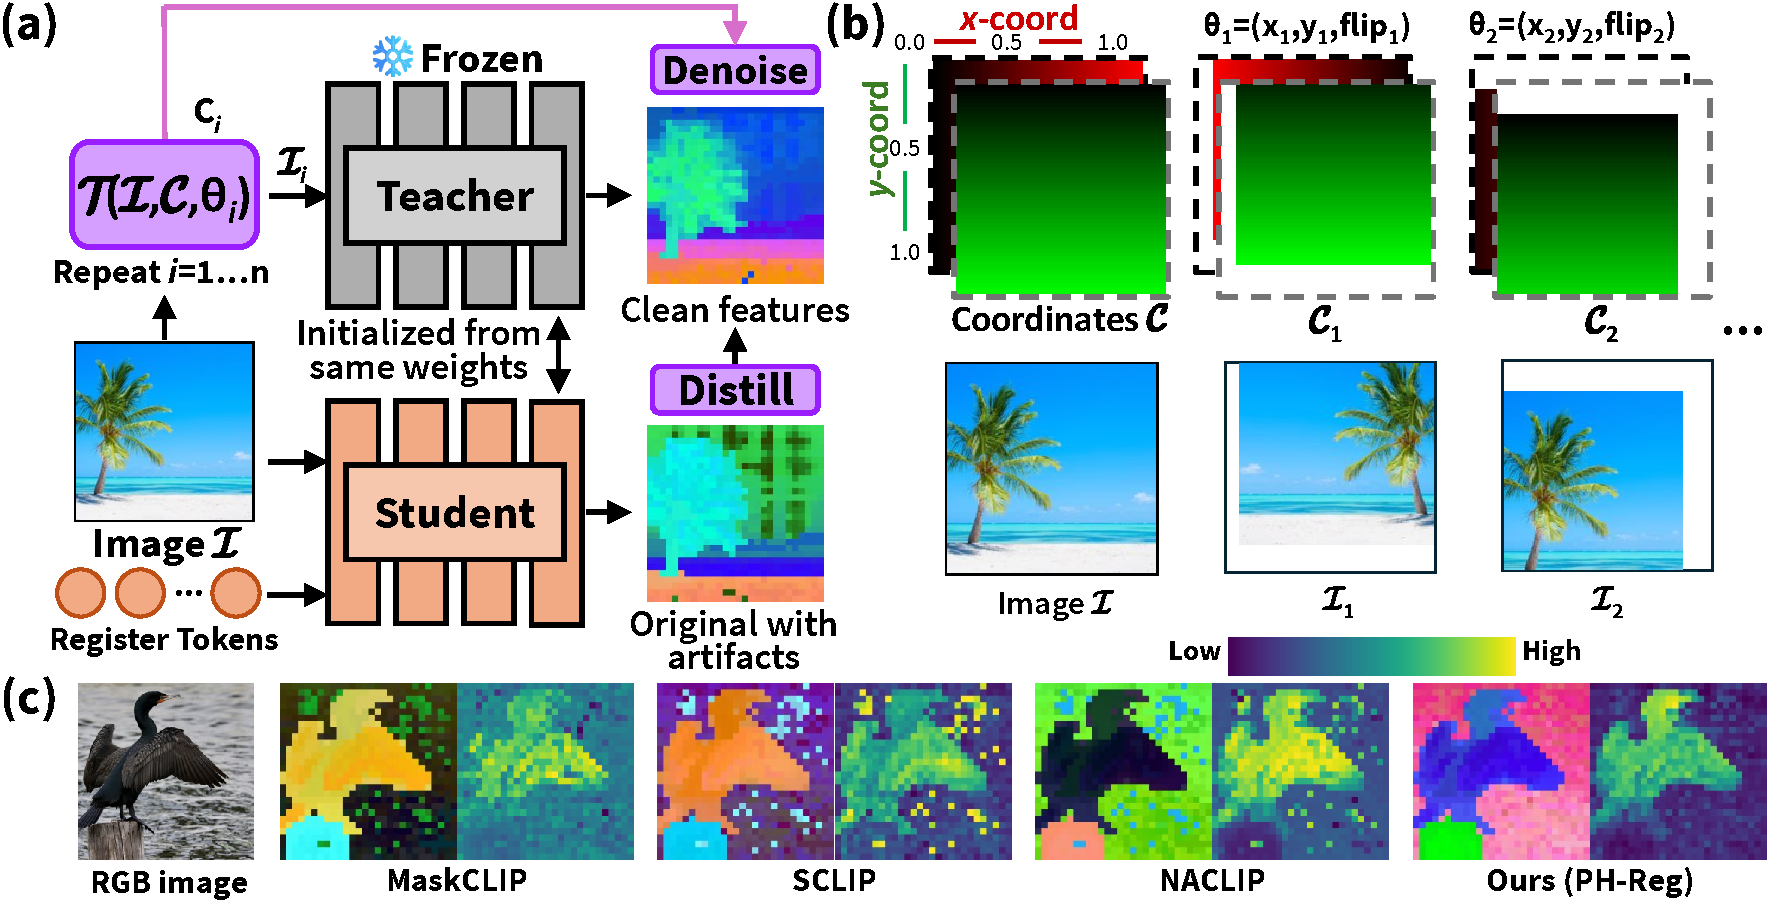
\includegraphics[width=1.0\linewidth]{fig_pdf/arch.pdf}
  \caption{\textbf{Learning Framework of PH-Reg.} \textbf{(a)} Our framework begins by creating two networks from the same set of weights. In the teacher, the weights are frozen and unmodified. In the student, the only additional parameters are learnable register tokens. The teacher creates a learning target using denoised representations. \textbf{(b)} An image $\mathcal{I}$ undergoes augmentation by function $\mathcal{T}$ with random augmentation parameters consisting of random offsets and horizontal flips.\textbf{(c)} Given an RGB image, we utilize UMAP to visualize the features, and a heatmap using CLIP text query. Our method can produce significantly cleaner dense representations with minimal additional inference cost.}
  \vspace{-.5cm}
  \label{fig:arch}
\end{figure}